% IEEE TALE 2026 — Short Paper (4 pages, A4, double-blind) — V2 (post-review revision)
% Compile: pdflatex tale2026_short_v2.tex (twice)
% Revision V1->V2 maps to the peer-review roadmap: see paper/CHANGELOG_v2.md.
\documentclass[conference,a4paper]{IEEEtran}
\usepackage[T1]{fontenc}
\usepackage[utf8]{inputenc}
\usepackage{graphicx}
\usepackage{booktabs}
\usepackage{tikz}
\usetikzlibrary{positioning,arrows.meta}
\usepackage{balance}
\usepackage[hidelinks]{hyperref}

% ===== BENCHMARK RESULT MACROS — mean +/- sample SD over k=5 runs =====
% PENDING k=5 RUN: the "+/- 0.0" below are PLACEHOLDER SDs and the means are the
% prior single-run values. After running bench/reliability_bench.mjs --repeat 5
% (see paper/RUN_PLAN_v2.md), replace every \s.../\a... macro string with the
% mean +/- SD read from bench/results-*/summary-stats.json
% (semanticValidityRate, spuriousActionRate, interceptedActions).
\newcommand{\bTotalCalls}{900} % 30 prompts x 6 configs (4B x4 cond + 12B + 70B) x 5 reps
% --- Table II (deployment scenarios, full pipeline): Spur / Valid / Interc ---
\newcommand{\sSPUmFour}{37.5\,$\pm$\,0.0}   \newcommand{\sVALmFour}{77.8\,$\pm$\,0.0}    \newcommand{\sINTmFour}{10\,$\pm$\,0.0}
\newcommand{\sSPUmTwelve}{0.0\,$\pm$\,0.0}  \newcommand{\sVALmTwelve}{66.7\,$\pm$\,0.0}  \newcommand{\sINTmTwelve}{12\,$\pm$\,0.0}
\newcommand{\sSPUmSeventy}{0.0\,$\pm$\,0.0} \newcommand{\sVALmSeventy}{80.0\,$\pm$\,0.0} \newcommand{\sINTmSeventy}{11\,$\pm$\,0.0}
% --- Table III (ablation, Gemma 3 4B local): Spur / Valid / Interc ---
\newcommand{\aSPUfull}{37.5\,$\pm$\,0.0}    \newcommand{\aVALfull}{77.8\,$\pm$\,0.0}     \newcommand{\aINTfull}{10\,$\pm$\,0.0}
\newcommand{\aSPUnoseed}{37.5\,$\pm$\,0.0}  \newcommand{\aVALnoseed}{92.0\,$\pm$\,0.0}   \newcommand{\aINTnoseed}{4\,$\pm$\,0.0}
\newcommand{\aSPUnoretry}{37.5\,$\pm$\,0.0} \newcommand{\aVALnoretry}{76.6\,$\pm$\,0.0}  \newcommand{\aINTnoretry}{11\,$\pm$\,0.0}
\newcommand{\aSPUnosys}{37.5\,$\pm$\,0.0}   \newcommand{\aVALnosys}{68.9\,$\pm$\,0.0}    \newcommand{\aINTnosys}{14\,$\pm$\,0.0}
% ============================================================================

\begin{document}

\title{Validate Before You Apply: An Action-Validation Layer for LLM Tutors that Act on Learner Artifacts in Computer Networks Education}

\author{\IEEEauthorblockN{Anonymous Author(s)}
\IEEEauthorblockA{Submission to IEEE TALE 2026 --- omitted for double-blind review}}

\maketitle

\begin{abstract}
Large language models (LLMs) promise adaptive tutoring, but when a tutoring agent can also act on the learner's working artifact, hallucination acquires a new cost: an incorrect action silently corrupts the very object the student is reasoning about. We present CAPA8, a browser-based environment for computer networks education that couples a conversational LLM tutor with an interactive network-topology simulator the tutor can read and modify. Its central design contribution is a pedagogical reliability layer: every model-proposed modification is expressed in a closed action grammar, parsed, and validated against the live topology state before it is applied, with ambiguous requests resolved by rule-based clarification dialogues that bypass the LLM entirely. Adaptive scaffolding is provided by a Level\,$\times$\,Focus mode matrix that reconfigures the tutor from step-by-step guidance to a technical peer. We make no claim about learning outcomes; the contribution is the design and its technical reliability. Because referential validation rejects any dangling reference by construction, our benchmark of \bTotalCalls{} model interactions across three deployment scenarios (two local open-weight models and a cloud-hosted model) does not test \emph{whether} invalid actions are caught but measures what makes the layer necessary: how often, and in which classes, models of differing capability emit invalid or spurious actions. Even a 70B cloud model proposes invalid actions on every run, while smaller models also emit spurious-but-well-formed ones that structural validation cannot see and a human-in-the-loop preview must cover. A classroom study is planned as future work.
\end{abstract}

\begin{IEEEkeywords}
large language models, intelligent tutoring systems, scaffolding, computer networks education, hallucination mitigation, human--AI collaboration
\end{IEEEkeywords}

\section{Introduction}
Computer networking is taught through abstractions---addressing, subnetting, routing, gateways---whose consequences only become visible when a concrete topology misbehaves. Professional simulators such as Cisco Packet Tracer~\cite{packettracer} and emulation environments such as Mininet~\cite{lantz2010mininet} give students that concreteness, but they carry steep learning curves, and none of them explains \emph{why} the ping the student just issued never arrived. The explanatory gap is usually filled by an instructor, who does not scale, or lately by a general-purpose chatbot, which cannot see the student's diagram and therefore reasons about a network that does not exist.

LLMs have shown clear potential as adaptive explainers in engineering education~\cite{kasneci2023chatgpt,denny2024computing}. The obvious next step---letting the tutor not only explain the student's artifact but also act on it---introduces a reliability problem that is qualitatively different from textual hallucination~\cite{ji2023survey}. A fabricated sentence can be challenged; a fabricated \emph{action} (connecting a PC to a router that does not exist, duplicating an IP address, ``fixing'' a missing gateway by adding a spurious cable) rewrites the learning artifact itself. Novices are the least equipped to detect such corruption: they cannot tell whether the inconsistency they now observe is their own misconception or the tool's error, which undermines both trust and the diagnostic reasoning the exercise was meant to train.

CAPA8 is a no-install, browser-based environment that addresses this problem by treating the LLM as an \emph{untrusted proposer}. The model never mutates the topology directly. It emits proposals in a closed action grammar; a deterministic pipeline classifies the student's intent before any model call, constrains the prompt, parses the response, validates every proposed action against the live graph state, and routes batches through a human-confirmable preview with single-step undo. The same pipeline carries the pedagogy: a Level\,$\times$\,Focus mode matrix adapts the depth and register of explanations, and a topology analyzer injects the same misconfiguration warnings the student sees on the canvas into the model's context, so tutor and student literally look at the same network.

This paper makes three contributions: (1)~the design of a validate-before-apply action pipeline as a pedagogical reliability mechanism for LLM tutors that operate on learner artifacts; (2)~an adaptive scaffolding scheme that operationalizes tutoring styles as a selectable Level\,$\times$\,Focus matrix combined with intent-dependent decoding temperature; and (3)~a preliminary technical evaluation---unit-test coverage of the deterministic pipeline plus a reliability benchmark over three deployment scenarios with an ablation of the prompt-side mechanisms---that, rather than re-deriving the tautology that a referential-integrity check rejects dangling references, quantifies the premise that makes such a check worthwhile: how often, and in which classes, LLMs of varying capability emit invalid or spurious actions. We evaluate reliability, not learning; comprehension and scaffolding effects await the classroom study (\S\ref{sec:concl}).

\section{Related Work}
\subsubsection*{LLMs in computing education}
Kasneci et al.~\cite{kasneci2023chatgpt} map the opportunities and risks of LLMs across education, identifying hallucination and overreliance as core concerns. Within computing education, Denny et al.~\cite{denny2024computing} survey the post-GPT landscape, and CodeHelp~\cite{liffiton2023codehelp} demonstrates guardrails that keep an LLM helper from emitting full solutions in programming classes. CodeHelp's guardrails shape the \emph{text} a model returns; CAPA8 extends the guardrail idea to \emph{state-changing actions}, where the failure mode is not an unwanted answer but a corrupted artifact.

\subsubsection*{Scaffolding and intelligent tutoring systems}
The tutor configurations in CAPA8 instantiate classic scaffolding theory: graduated assistance within the learner's zone of proximal development~\cite{vygotsky1978mind,wood1976role}, software realizations of structuring and problematizing supports~\cite{reiser2004scaffolding}, and the ITS tradition of step-based adaptive dialogue~\cite{vanlehn2011relative}. CAPA8 differs from end-to-end LLM tutors in deliberately keeping parts of the dialogue deterministic: ambiguity resolution and misconfiguration detection are rule-based, reserving the LLM for explanation and proposal generation.

\subsubsection*{Constraining LLMs that act}
Hallucination surveys~\cite{ji2023survey} motivate a growing toolbox of output constraints, from programmable conversational rails to constrained semantic decoding~\cite{rebedea2023nemo}. Letting models \emph{act} through tools is by now standard---reason-and-act loops~\cite{yao2023react} and large function-calling repertoires~\cite{qin2023toolllm}---and such agents are increasingly placed in educational roles~\cite{jin2024teachable}. These mechanisms, including native JSON and function-calling modes, constrain the \emph{syntax} of a call at generation time; they are stateless with respect to the application and cannot know that \emph{Router5} is absent from \emph{this} graph or that an address is already in use. CAPA8 adds a complementary, state-dependent stage: semantic validation of each proposed action against the live topology (referential integrity, duplicate addresses, type normalization), plus a human confirmation step consistent with human--AI interaction guidelines~\cite{amershi2019guidelines}. Validate-before-apply is thus not novel in the abstract; our contribution is its instantiation as a pedagogical reliability layer in an artifact-centric tutor, where a rejected action prevents a corrupted \emph{learning} object rather than a failed API call. To our knowledge this has not been reported for network-education tools, whose mainstream representatives~\cite{packettracer,lantz2010mininet} offer no integrated conversational tutoring at all.

\section{System Design}
\subsection{Architecture Overview}
CAPA8 is a dependency-light web app (vanilla ES6 modules, no build step) with two surfaces sharing one conversation store: a chat page and a topology simulator with an embedded tutor panel. The simulator offers ten device types (routers through industrial PLCs), configurable links, an animated virtual terminal (\texttt{ping}, \texttt{traceroute}, \texttt{ipconfig}, ARP, routing), and eleven example topologies; a Node.js backend relays prompts to a cloud provider or a locally hosted open-weight model, so the whole stack runs on commodity hardware without sending student data to third parties.

Two design decisions tie the architecture to pedagogy. A static topology analyzer continuously detects eight classes of misconfiguration (duplicate IPs, isolated nodes, missing gateways, downed links) and renders them to the student, and the identical issue list is serialized into the LLM context, so tutor and student reason over the same evidence. Conversation state also persists across both surfaces.

\begin{figure}[!tb]
\centering
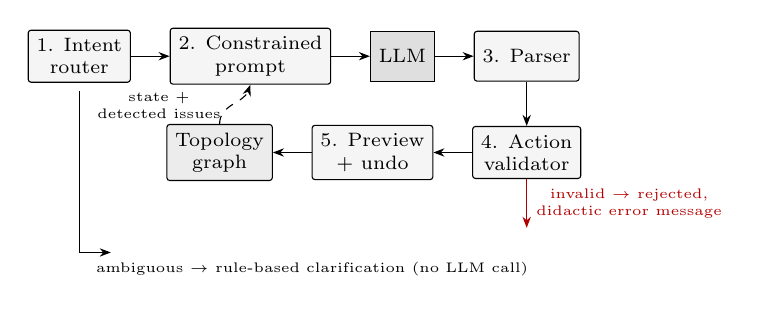
\begin{tikzpicture}[
  font=\scriptsize,
  stage/.style={draw, rounded corners=1pt, align=center, inner sep=3pt, minimum height=18pt, fill=gray!8},
  llm/.style={draw, align=center, inner sep=3pt, minimum height=18pt, fill=gray!25},
  arr/.style={-{Stealth[length=4pt]}},
  lbl/.style={font=\tiny, align=center},
  node distance=10pt and 14pt]
\node[stage] (intent) {1. Intent\\router};
\node[stage, right=of intent] (prompt) {2. Constrained\\prompt};
\node[llm, right=of prompt] (llm) {LLM};
\node[stage, right=of llm] (parse) {3. Parser};
\node[stage, below=16pt of parse] (valid) {4. Action\\validator};
\node[stage, left=of valid] (preview) {5. Preview\\+ undo};
\node[stage, left=of preview, fill=gray!15] (graph) {Topology\\graph};
\draw[arr] (intent) -- (prompt);
\draw[arr] (prompt) -- (llm);
\draw[arr] (llm) -- (parse);
\draw[arr] (parse) -- (valid);
\draw[arr] (valid) -- (preview);
\draw[arr] (preview) -- (graph);
\draw[arr, dashed] (graph.north) to[out=90,in=-110] node[lbl, left, pos=0.45]{state +\\detected issues} (prompt.south);
\draw[arr] ([yshift=-3pt]intent.south) |- node[lbl, below right=0pt and -2pt, pos=0.7]{ambiguous $\to$ rule-based clarification (no LLM call)} ++(0.4,-2.05);
\draw[arr, red!70!black] (valid.south) -- node[lbl, right, text=red!70!black]{invalid $\to$ rejected,\\didactic error message} ++(0,-0.62);
\end{tikzpicture}
\caption{The validate-before-apply pipeline. The LLM only proposes; deterministic stages decide what reaches the learner's topology.}
\label{fig:pipeline}
\end{figure}

\subsection{Adaptive Scaffolding: the Level\texorpdfstring{\,$\times$\,}{x}Focus Matrix}
Tutoring style is the product of a three-step \emph{Level} and a two-value \emph{Focus} (Table~\ref{tab:modes}), yielding six configurations compiled into the system prompt. Levels encode graduated, fadeable scaffolding~\cite{wood1976role,reiser2004scaffolding}---from a guided novice register that bans unexplained acronyms and closes each turn with a reflection question, to a technical peer register that cites RFC/IEEE standards---while Focus selects the task frame, design or troubleshoot. Decoding temperature is additionally bound to intent---0.0 for modifications, 0.2 for conceptual explanation---so creative variability is spent on pedagogy, never on state changes.

\begin{table}[!tb]
\caption{Scaffolding configurations (Level $\times$ Focus)}
\label{tab:modes}
\centering
\scriptsize
\begin{tabular}{@{}lp{6.0cm}@{}}
\toprule
\textbf{Level} & \textbf{Tutor behavior (applies to both foci)} \\
\midrule
Guided    & Step-by-step; analogies; no unexplained acronyms; flags novice errors; ends with a reflection question. \\
Balanced  & Direct and practical; at most three paragraphs or a short list. \\
Technical & Dense, standards-referenced (RFC/IEEE); peer register. \\
\midrule
\textbf{Focus} & \emph{Design}: propose and build topologies.\quad \emph{Troubleshoot}: analyze the graph and explain faults. \\
\bottomrule
\end{tabular}
\end{table}

\subsection{Deterministic Intent Routing and Clarification}
Before any model call, a rule-based classifier assigns each utterance one of six intents (conceptual, graph query, diagnostic, clear or ambiguous modification, full-graph application). It uses verb lexicons, question patterns, and the live graph: a message is a \emph{clear} modification only if it references an existing node or concrete target. Ambiguous requests (``add a device somewhere'') never reach the LLM; a clarification dialogue is instead generated from the graph, offering the available attachment points. This keeps such interactions instant, free, and predictable~\cite{vanlehn2011relative}, and sets downstream policy: prompt blocks, temperature, and whether the action grammar is enabled.

\subsection{Action Grammar and the Validation Layer}
All state changes use a closed grammar of seven actions (add, update, and delete for nodes and links; set link status; apply graph) serialized as JSON inside explicit \texttt{[CAPA8\_ACTION]} delimiters. Three prompt-side mechanisms raise the chance an action request yields well-formed blocks: a directive with paired wrong/correct counter-examples (gateway repair must patch a node property, never add a cable), canonical examples seeded only for action intents, and a single stricter retry when an expected action is missing.

What the model returns is still untrusted. A parser isolates the delimited blocks (malformed JSON is marked invalid and can never execute), and each surviving action passes semantic validation against the current graph: the action type must be whitelisted; referenced nodes must exist; duplicate IPs and links are flagged; unknown device types are normalized through an alias table; and an \texttt{add\_node} naming an existing node is rewritten into an \texttt{update\_node}, converting the commonest duplication hallucination into the action the model should have chosen. Rejected actions are not dropped silently: the validator emits an explanatory message (``source node \emph{Router5} not found''), turning the failure into feedback for the student and the model.

\subsection{Human-in-the-Loop Application}
\label{sec:hitl}
Validated actions still require consent at the right granularity. Batches of three or more actions open a preview panel for review and confirmation; any applied batch is one atomic undo step; and the frontend ignores model-proposed coordinates, keeping layout authority on the client. Following human--AI interaction guidance on efficient correction and graceful degradation~\cite{amershi2019guidelines}, the tutor's agency is visible, bounded, and reversible---preconditions, we argue, for trusting an acting tutor in a classroom.

\section{Preliminary Evaluation}
\subsection{Unit-Test Coverage of the Deterministic Pipeline}
The deterministic pipeline components are covered by 47 unit tests (validator, intent router, response parser, graph model), all passing. The validator tests exercise the properties the reliability argument rests on: nonexistent references and unknown action/device types are rejected, alias normalization and the \texttt{add\_node}-to-\texttt{update\_node} rewrite behave as specified, and duplicate IPs raise warnings. These are unit tests, not formal proofs, but they pin down the deterministic behavior the by-construction interception argument below relies on.

\subsection{Reliability Benchmark}
We probed the pipeline with a scripted benchmark of 30 student-style Spanish utterances against a fixed five-node topology seeded with deliberate faults (a PC without gateway, a PC without IP, an in-use IP). The suite has 16 clear modification requests (including gateway-repair, IP-assignment, nonexistent-device, and occupied-IP traps), 6 diagnostic requests, and 8 conceptual or query utterances for which any emitted action is spurious. Every response was parsed and validated by the production code itself, and the full suite was repeated five times per configuration (\bTotalCalls{} interactions in all); tables report mean\,$\pm$\,SD across the five runs. In every run, all 16 modification prompts yielded a parseable action and every block was well-formed JSON (action-emission and JSON-validity were 100\% throughout); we omit these non-discriminating columns and report the three quantities that vary---spurious-action rate, semantic validity, and intercepted actions.

\subsubsection*{Across deployment scenarios}
We ran the full pipeline under three scenarios spanning the privacy/cost spectrum a school faces: a small local model (Gemma~3~4B~\cite{gemmateam2025gemma3}), a larger local model (Gemma~3~12B), both served through Ollama on commodity hardware, and a cloud-hosted high-capacity model (Llama~3.3~70B via Groq). Because referential validation cannot admit a dangling reference, interception is guaranteed \emph{by construction}; the benchmark therefore does not test \emph{whether} invalid actions are caught but measures the premise that justifies the layer---the rate and classes of actions it must absorb (Table~\ref{tab:models}). None of the three models is free of \emph{semantically} invalid actions: each produced roughly ten to twelve that referenced a nonexistent node or duplicated an address, all intercepted, and even the 70B cloud model did so on every run. What capability changes is the \emph{second} failure mode, the one validation cannot cover: an action that is well-formed and references real nodes yet is contextually \emph{spurious}---emitted in reply to a purely conceptual question. The 4B model does this on 37.5\% of conceptual prompts; the 12B and 70B never do. Such actions pass every structural check and would reach the learner's graph but for the human-confirmable preview and atomic undo of Section~\ref{sec:hitl}; the two safeguards are complementary, and a smaller model shifts load from the automatic one onto the human one (\S\ref{sec:disc}).

\begin{table}[!tb]
\caption{Full pipeline across deployment scenarios (30 prompts $\times$ 5 runs)}
\label{tab:models}
\centering
\scriptsize
\begin{tabular}{@{}llccc@{}}
\toprule
\textbf{Model} & \textbf{Deploy.} & \textbf{Spur.\,\%} & \textbf{Valid\,\%} & \textbf{Interc.} \\
\midrule
Gemma 3 4B    & Local & \sSPUmFour    & \sVALmFour    & \sINTmFour \\
Gemma 3 12B   & Local & \sSPUmTwelve  & \sVALmTwelve  & \sINTmTwelve \\
Llama 3.3 70B & Cloud & \sSPUmSeventy & \sVALmSeventy & \sINTmSeventy \\
\bottomrule
\multicolumn{5}{@{}p{8.2cm}@{}}{\tiny Mean\,$\pm$\,SD over five runs. Spur.: \% of the 8 conceptual/query prompts wrongly answered with an action. Valid: \% of parsed actions passing semantic validation. Interc.: invalid actions caught before reaching the graph. Action-emission and JSON-validity rates were 100\% in every run (omitted). The three scenarios confound model family, size, and host; we read them as deployment options, not a controlled capability comparison (see \S\ref{sec:disc}).}
\end{tabular}
\end{table}

\subsubsection*{Ablation of the prompt-side mechanisms}
To isolate each prompt-side mechanism we ablated them on the smallest and hardest case, Gemma~3~4B, where structured-output reliability is most fragile: the full pipeline, no seeded examples, no auto-retry, and the directive moved from the system channel into the user prompt (Table~\ref{tab:bench}). Routing the directive through the system channel is the dominant aid: removing it is the largest single degradation in the table, maximizing the count of invalid actions the validator must intercept and minimizing semantic validity. The seeded examples and auto-retry show no clear benefit at this model size---the model already emits an action for every request, so the retry never fires---a candid result we report rather than overstate. The validator's interception nevertheless holds across all four conditions and all runs.

\begin{table}[!tb]
\caption{Ablation of prompt-side mechanisms, Gemma 3 4B local (30 prompts $\times$ 5 runs per condition)}
\label{tab:bench}
\centering
\scriptsize
\begin{tabular}{@{}lccc@{}}
\toprule
\textbf{Condition} & \textbf{Spur.\,\%} & \textbf{Valid\,\%} & \textbf{Interc.} \\
\midrule
Full pipeline & \aSPUfull & \aVALfull & \aINTfull \\
-- seeded examples & \aSPUnoseed & \aVALnoseed & \aINTnoseed \\
-- auto-retry & \aSPUnoretry & \aVALnoretry & \aINTnoretry \\
-- system channel & \aSPUnosys & \aVALnosys & \aINTnosys \\
\bottomrule
\multicolumn{4}{@{}p{8.2cm}@{}}{\tiny Mean\,$\pm$\,SD over five runs. Columns as in Table~\ref{tab:models}. Action-emission and JSON-validity rates were 100\% in every condition and run (omitted). Interc.: invalid actions intercepted by the validator that would otherwise have corrupted the graph.}
\end{tabular}
\end{table}

\section{Discussion and Limitations}
\label{sec:disc}
The validation layer guarantees \emph{structural} soundness, not pedagogical optimality, and two failure modes survive it. First, an action can be structurally valid yet didactically wrong: connecting PC1 to the router with a new cable (the gateway trap) is referentially valid but pedagogically incorrect, and only the counter-example prompts, not the validator, steer the model away from it; encoding such domain-pedagogical rules as first-class validations is a natural next step. Second, the spurious-action mode quantified above (37.5\% of conceptual prompts for the 4B model) is structurally valid by definition and passes the validator untouched, so only the human-in-the-loop preview and undo stand in its way. A validator that silently absorbs every malformed action also risks \emph{automation complacency}---a student who never sees a rejection may trust whatever is applied---which is why CAPA8 surfaces rejections as visible, didactic events rather than silent drops.

The benchmark has clear scope limits: it covers three models, one seeded topology, and Spanish utterances only, and it measures reliability, not learning. The three deployment scenarios moreover confound model family, size, and host (Gemma vs.\ Llama; 4B/12B vs.\ 70B; local vs.\ cloud), so they should be read as deployment options a school might select rather than a controlled capability comparison; isolating any single factor would need a crossed design we did not run. No claims about learning outcomes are made; comprehension, trust calibration, and scaffolding-level effects require the classroom study below. Finally, we \emph{conjecture}---without yet testing it---that validate-before-apply extends to other artifact-centric subjects (electronic circuits, database schemas, chemical process diagrams), wherever an LLM tutor may touch the thing the student is building.

\section{Conclusion and Future Work}
\label{sec:concl}
CAPA8 demonstrates that an LLM tutor can be given hands---the ability to construct and repair the learner's network topology---without inheriting the model's unreliability, by interposing deterministic intent routing, a closed action grammar, state-aware semantic validation, and human-confirmable application between proposal and effect. The interception of structurally invalid actions is guaranteed by construction; our preliminary technical evidence (47 passing unit tests; a \bTotalCalls-interaction benchmark spanning local 4B and 12B models and a 70B cloud model, five runs each) instead characterizes what that layer must absorb: every model, the 70B cloud model included, proposes invalid actions on every run, while smaller models additionally emit spurious actions on conceptual prompts---a class structural validation cannot see and that the human-in-the-loop step exists to cover. The architecture runs on hardware schools already own. The next step is a controlled classroom study with networking students (pre/post concept inventory, usability, and scaffolding-level comparison), to be conducted under institutional ethics review. This paper reports no human-subjects data.

\section*{Acknowledgment}
\textit{AI-use disclosure (per IEEE/TALE policy):} a generative AI system (Claude, Anthropic) assisted with text editing, benchmark scripting, and LaTeX formatting under the authors' direction; the authors reviewed and verified all content, code, and results, take full responsibility, and designed and implemented CAPA8 themselves. [Author names, affiliations, funding, and the code repository are withheld for double-blind review and restored upon acceptance.]

\balance
\footnotesize
\begin{thebibliography}{16}
\bibitem{kasneci2023chatgpt} E. Kasneci \emph{et al.}, ``ChatGPT for good? On opportunities and challenges of large language models for education,'' \emph{Learning and Individual Differences}, vol. 103, p. 102274, 2023.
\bibitem{denny2024computing} P. Denny \emph{et al.}, ``Computing education in the era of generative AI,'' \emph{Communications of the ACM}, vol. 67, no. 2, pp. 56--67, 2024.
\bibitem{liffiton2023codehelp} M. Liffiton, B. Sheese, J. Savelka, and P. Denny, ``CodeHelp: Using large language models with guardrails for scalable support in programming classes,'' in \emph{Proc. 23rd Koli Calling Int. Conf. on Computing Education Research}, 2023, pp. 1--11.
\bibitem{ji2023survey} Z. Ji \emph{et al.}, ``Survey of hallucination in natural language generation,'' \emph{ACM Computing Surveys}, vol. 55, no. 12, pp. 1--38, 2023.
\bibitem{vygotsky1978mind} L. S. Vygotsky, \emph{Mind in Society: The Development of Higher Psychological Processes}. Cambridge, MA: Harvard University Press, 1978.
\bibitem{wood1976role} D. Wood, J. S. Bruner, and G. Ross, ``The role of tutoring in problem solving,'' \emph{Journal of Child Psychology and Psychiatry}, vol. 17, no. 2, pp. 89--100, 1976.
\bibitem{reiser2004scaffolding} B. J. Reiser, ``Scaffolding complex learning: The mechanisms of structuring and problematizing student work,'' \emph{Journal of the Learning Sciences}, vol. 13, no. 3, pp. 273--304, 2004.
\bibitem{vanlehn2011relative} K. VanLehn, ``The relative effectiveness of human tutoring, intelligent tutoring systems, and other tutoring systems,'' \emph{Educational Psychologist}, vol. 46, no. 4, pp. 197--221, 2011.
\bibitem{rebedea2023nemo} T. Rebedea, R. Dinu, M. Sreedhar, C. Parisien, and J. Cohen, ``NeMo Guardrails: A toolkit for controllable and safe LLM applications with programmable rails,'' in \emph{Proc. EMNLP 2023: System Demonstrations}, 2023, pp. 431--445.
\bibitem{amershi2019guidelines} S. Amershi \emph{et al.}, ``Guidelines for human--AI interaction,'' in \emph{Proc. CHI Conf. on Human Factors in Computing Systems}, 2019, pp. 1--13.
\bibitem{yao2023react} S. Yao, J. Zhao, D. Yu, N. Du, I. Shafran, K. Narasimhan, and Y. Cao, ``ReAct: Synergizing reasoning and acting in language models,'' in \emph{Proc. Int. Conf. on Learning Representations (ICLR)}, 2023.
\bibitem{qin2023toolllm} Y. Qin \emph{et al.}, ``ToolLLM: Facilitating large language models to master 16000+ real-world APIs,'' \emph{arXiv preprint arXiv:2307.16789}, 2023.
\bibitem{jin2024teachable} H. Jin, S. Lee, H. Shin, and J. Kim, ``Teach AI how to code: Using large language models as teachable agents for programming education,'' in \emph{Proc. CHI Conf. on Human Factors in Computing Systems}, 2024, pp. 1--28.
\bibitem{packettracer} Cisco Networking Academy, ``Cisco Packet Tracer,'' 2024. [Online]. Available: \url{https://www.netacad.com/courses/packet-tracer}
\bibitem{lantz2010mininet} B. Lantz, B. Heller, and N. McKeown, ``A network in a laptop: Rapid prototyping for software-defined networks,'' in \emph{Proc. 9th ACM SIGCOMM Workshop on Hot Topics in Networks (HotNets-IX)}, 2010, pp. 1--6.
\bibitem{gemmateam2025gemma3} Gemma Team, Google DeepMind, ``Gemma 3 technical report,'' \emph{arXiv preprint arXiv:2503.19786}, 2025.
\end{thebibliography}

\end{document}
